\documentclass[presentation,sansserif]{beamer}
\usefonttheme[onlymath]{serif}
%\renewcommand\mathfamilydefault{ppl}
%\usetheme{Warsaw}
%\usecolortheme{beetle}
\usepackage {mathpazo}
\usepackage{graphicx}
\usepackage{blindtext}
\usepackage{xfrac}

\title[Developing pop-gen models for polyploids]{Developing models for genotype uncertainty, inbreeding, and allelic inheritance in non-model polyploids}
\author[Blischak \textit{et al}.]{Paul Blischak$^1$ :: Laura Kubatko$^{1,2}$ :: Andrea Wolfe$^1$}

\date{}

\definecolor{itemcol}{RGB}{0,128,255}
\definecolor{back}{RGB}{1,22,39}
\definecolor{alert}{RGB}{255,0,81}
\definecolor{yell}{RGB}{255,222,0}
\setbeamercolor{alerted text}{fg=alert}
\setbeamercolor{section in toc}{fg=black, bg=black}
\setbeamercolor{item}{fg=itemcol,bg=itemcol}
\setbeamercolor{structure}{fg=itemcol!95!black}
\setbeamercolor{background canvas}{bg=white!15!black}
\setbeamercolor{normal text}{fg=white!95!black, bg=white!95!black}
\setbeamercolor{math text}{fg=white, bg=white}

\newcommand{\inline}[1]{\fcolorbox{white!15!black}{white!20!black}{\texttt{#1}}}

\begin{document}

\beamertemplatenavigationsymbolsempty

\begin{frame}[plain]
	\vspace{-1.2in}
	\titlepage
	
	\vspace{-1.2in}
	\begin{center}
	
		{\footnotesize Ohio State University 	
		\vspace{0.05in}
		
		$^1$Department of EEOB :: $^2$Department of Statistics
		}		
	\end{center}
	\vspace{-0.2in}
		
\end{frame}


\begin{frame}[t]{Contemporary polyploidy}
  \vspace{0.3in}
  \pause
  
  Recent whole genome duplication has been an important force in the evolution of many groups.
  \vspace{0.3in}
  \pause
  
  \textbf{More than just plants}.
  \vspace{0.3in}
  \pause
    
  It is also common in several lineages of amphibians, fish, fungi, and others.

\end{frame}

\begin{frame}[t]{Contemporary polyploidy}
\framesubtitle{Basic types of polyploids}

	\onslide<2->{\textbf{Autopolyploids}:}

	\begin{center}
		\onslide<3->{
\includegraphics[width=0.5\textwidth]{eps/autopolyploid-formation}}
	\end{center}
	
	\onslide<2->{\textbf{Allopolyploids}:}
	
	\begin{center}
		\onslide<4->{
\includegraphics[width=0.5\textwidth]{eps/allopolyploid-formation}}
	\end{center}

\end{frame}

\begin{frame}[t]{Non-model polyploids}
  \vspace{0.1in}

  The majority of polyploid organisms have little to no genomic resources available. \pause What do we do?
  \vspace{0.3in}
  \pause
  
  Techniques such as RAD sequencing have had success in non-model diploids---and polyploids too in some cases---but it is not nearly as common.
  \vspace{0.3in}
  \pause
  
  \textbf{The main problem}: what can we do if we collect RAD data for a polyploid that we know almost nothing about?
  \vspace{0.3in}
  \pause
  
  \textbf{We need methods...}

\end{frame}

\begin{frame}[t]{Polyploid pop-gen}

  \vspace{0.1in}
  A simple model for genotypes and allele frequencies:
  \vspace{0.2in}
  
	$D$ -- HTS data (reads and error values)
	
	$m$ -- ploidy-level
	
	$G$ -- genotype $(0,\dots,m)$
	
	$p$ -- allele frequency
		
	\pause
	\begin{equation*}
		\onslide<2->{\mathcal{L}(G) = P(D|G)^*.}
	\end{equation*}
	\vspace{-0.2in}
	
	\begin{equation*}
		\onslide<3->{\mathcal{L}(p) = P(D|p) = \sum_G P(D|G)P(G|p),}
	\end{equation*}
	\vspace{-0.2in}
	
	\begin{equation*}
		\onslide<4->{= \sum_G \mathcal{L}(G)P(G|p).}
	\end{equation*}
	
	\onslide<2->{\hfill {\tiny $^*$ genotype likelihood -- can be calculated with GATK\\ \hfill using loci clustered with PyRAD, for example}}

\end{frame}

\begin{frame}[t]{Assumptions}

  \begin{enumerate}
    \setlength\itemsep{0.25in}
    \item Hardy-Weinberg equilibrium (HWE).
    \item Loci are unlinked and independent.
    \item Genotypes are drawn from a single pool of alleles $=$ allelic inheritance pattern for autopolyploid.
  \end{enumerate}
  \vspace{0.25in}
  \pause

Mixed mating systems and double reduction can make HWE a poor assumption in autopolyploids \pause $\rightarrow$ inbreeding and increased homozygosity.
\vspace{0.25in}
\pause

Allopolyploids inherit two($+$) sets of chromosomes with different ancestries \pause $\rightarrow$ assuming draws from a single allele pool does not reflect their hybrid origin.

\end{frame}

\begin{frame}[t]{Modeling inheritance patterns}
\vspace{0.2in}
\pause

  Among the most difficult challenges for analyzing polyploid data.
  \vspace{0.3in}
  \pause
  
  The models we propose here attempt to be simple solutions to the many processes that likely affect inheritance in polyploids.
  \vspace{0.3in}
  \pause
  
  We do this using $F$-models for genetic correlations.
  \vspace{0.3in}
  \pause
  
  	\begin{enumerate}
		\item Inbreeding/disequilibrium in autopolyploids.
		\item Subgenome allele frequencies in allopolyploids.
	\end{enumerate}

\end{frame}

\begin{frame}[t]{A disequilibrium model for autopolyploids}

  In most models, $P(G|p)$ is binomially distributed $\rightarrow$ genotypes are in HW proportions.
  \vspace{0.3in}
  \pause
  
  To relax this, we use a different probability distribution for genotypes: the beta-binomial.
  \vspace{0.3in}
  \pause
  
  Using an additional parameter, $\phi$, the probability distribution for genotypes becomes
  \vspace{0.1in}
  
  \begin{equation}
    P(G=a|p,\phi) = \frac{\mathcal{B}(a + p\phi, m - a + (1-p)\phi)}{\mathcal{B}(p\phi, (1-p)\phi)},
  \end{equation}
  \vspace{0.2in}

  

with $a = 1,\dots,m$. \pause Here, $\mathcal{B}()$ is the beta function, and $\phi$ is related to the inbreeding coefficient as $F = \sfrac{1}{(1+\phi)}$.

\end{frame}

{ \setbeamercolor{background canvas}{bg=white!20!black} \setbeamercolor{math text}{bg=itemcol, fg=itemcol}
\begin{frame}[c,plain]{The effect of $F$ on the distribution genotypes}
\pause

  \begin{center}
    \frame{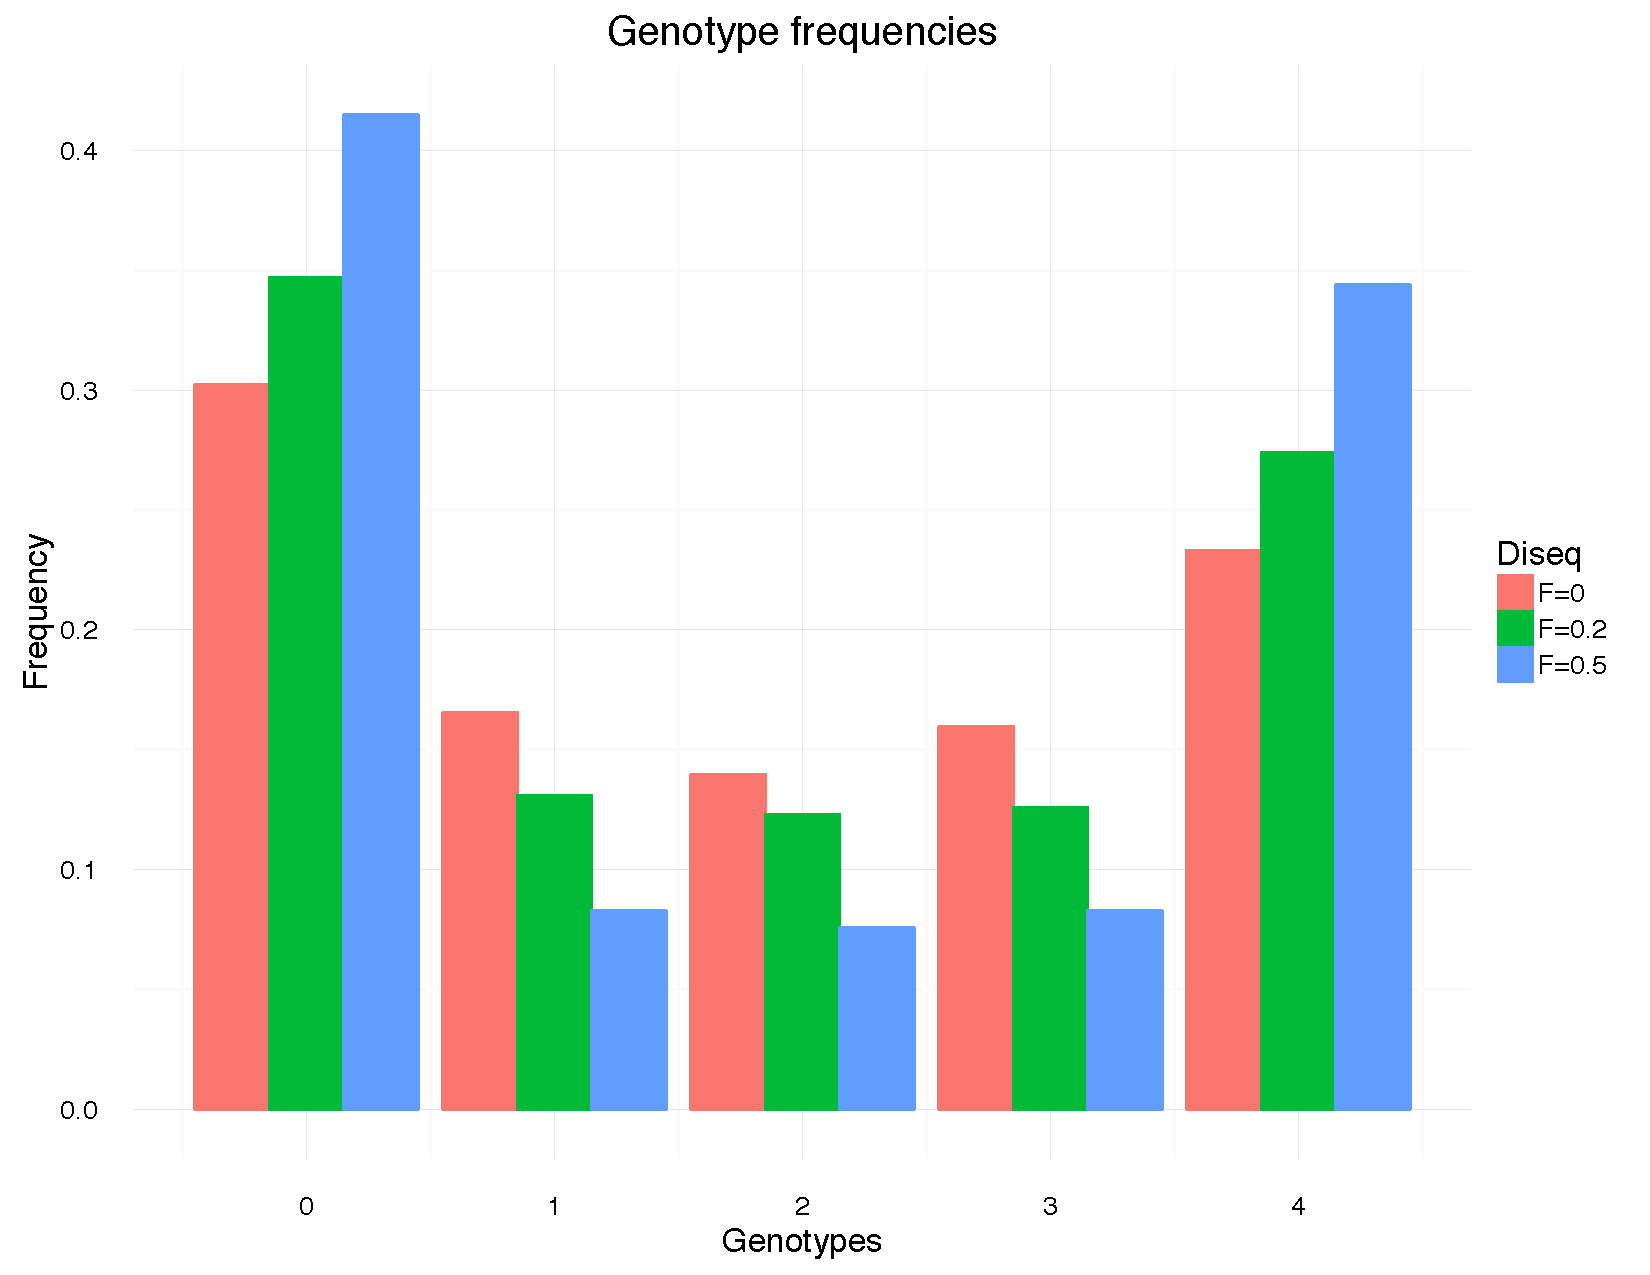
\includegraphics[width=0.9\textwidth]{pdf/genotype-freqs-diseq}}
  \end{center}
  
\end{frame}

}

{ \setbeamercolor{background canvas}{bg=white!20!black} \setbeamercolor{math text}{bg=itemcol, fg=itemcol}
\begin{frame}[c,plain]{Likelihood surface for $F$ and $p$}
\pause
	\framesubtitle{\hspace{15pt}}
	\begin{center}
		\frame{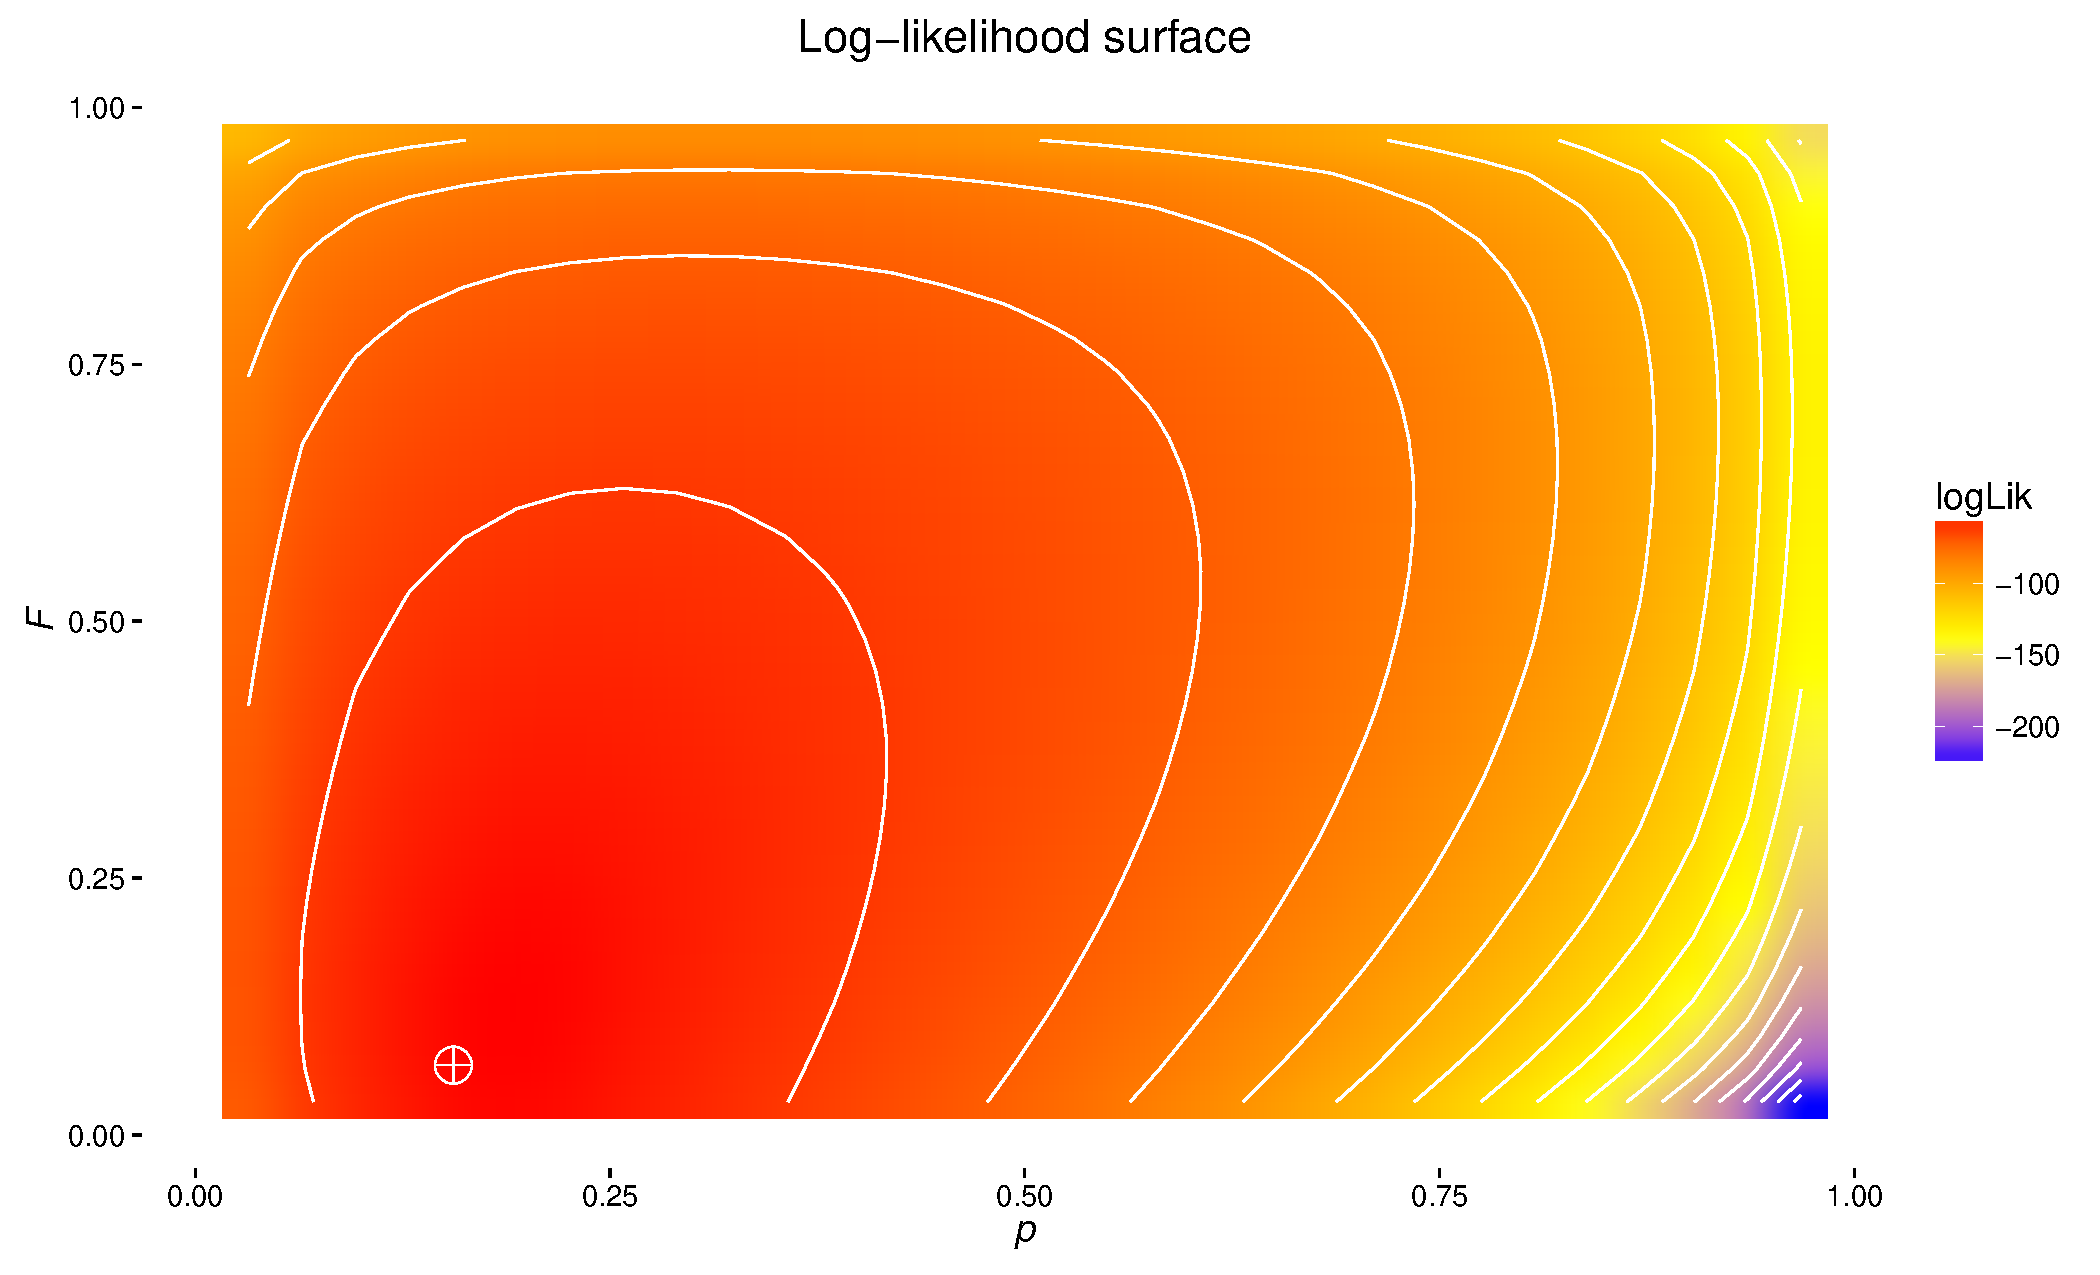
\includegraphics[width=\textwidth]{pdf/freq-phi-lik-surf2}}
	\end{center}
\end{frame}
}

\begin{frame}[t]{A subgenome model for allopolyploids}

Switching gears to allopolyploids, \pause consider the simple case of two subgenomes with different ancestry that are independent.
\vspace{0.3in}
\pause

We use a commonly employed $F$-model for correlated allele frequencies in the two subgenomes: divergence from a common ancestor with drift.
\vspace{0.3in}
\pause


$\pi$ -- ancestral allele frequency\\
$\theta$ -- drift [related to $F_{st} = 1/(1+\theta)$] \\
$p_1,p_2$ -- allele frequencies in subgenome one and two\\
\vspace{0.3in}
\pause

\begin{equation}
p_i|\pi,\theta \sim \text{beta}(\pi\theta,(1-\pi)\theta), \quad \text{for } i=1,2.
\end{equation}

\end{frame}

\begin{frame}[t]{A subgenome model for allopolyploids}

Genotypes in this case are a mixture of draws from the two subgenomes, each with a potentially different allele frequency.
\vspace{0.25in}
\pause

Given the ploidy of the two subgenomes ($m_1$,$m_2$), the genotype can be modeled as a sum of two binomially distributed random variable.
\vspace{0.25in}
\pause

This is a special case of the poisson-binomial distribution.
\pause

\begin{align}
P(G&=a|p_1,p_2,m_1,m_2) \nonumber \\[0.05in]
&= P(G=i|p_1,m_1) + P(G=j|p_2,m_2), \nonumber \\[0.05in]
&\text{ for } i=1,\dots,m_1; \; j=1,\ldots,m_2; \; i+j=a,
\end{align}

\vspace{-0.1in}
with $a = 0,\dots,m_1+m_2$.

\end{frame}

{ \setbeamercolor{background canvas}{bg=white!20!black} %\setbeamercolor{math text}{bg=itemcol, fg=itemcol}
\begin{frame}[c,plain]{\setbeamercolor{math text}{fg=itemcol, bg=itemcol}Likelihood surface for $p_1$ and $p_2$: low drift}

	\framesubtitle{$F_{st}=0.1$}
	\pause
	\begin{center}
		\frame{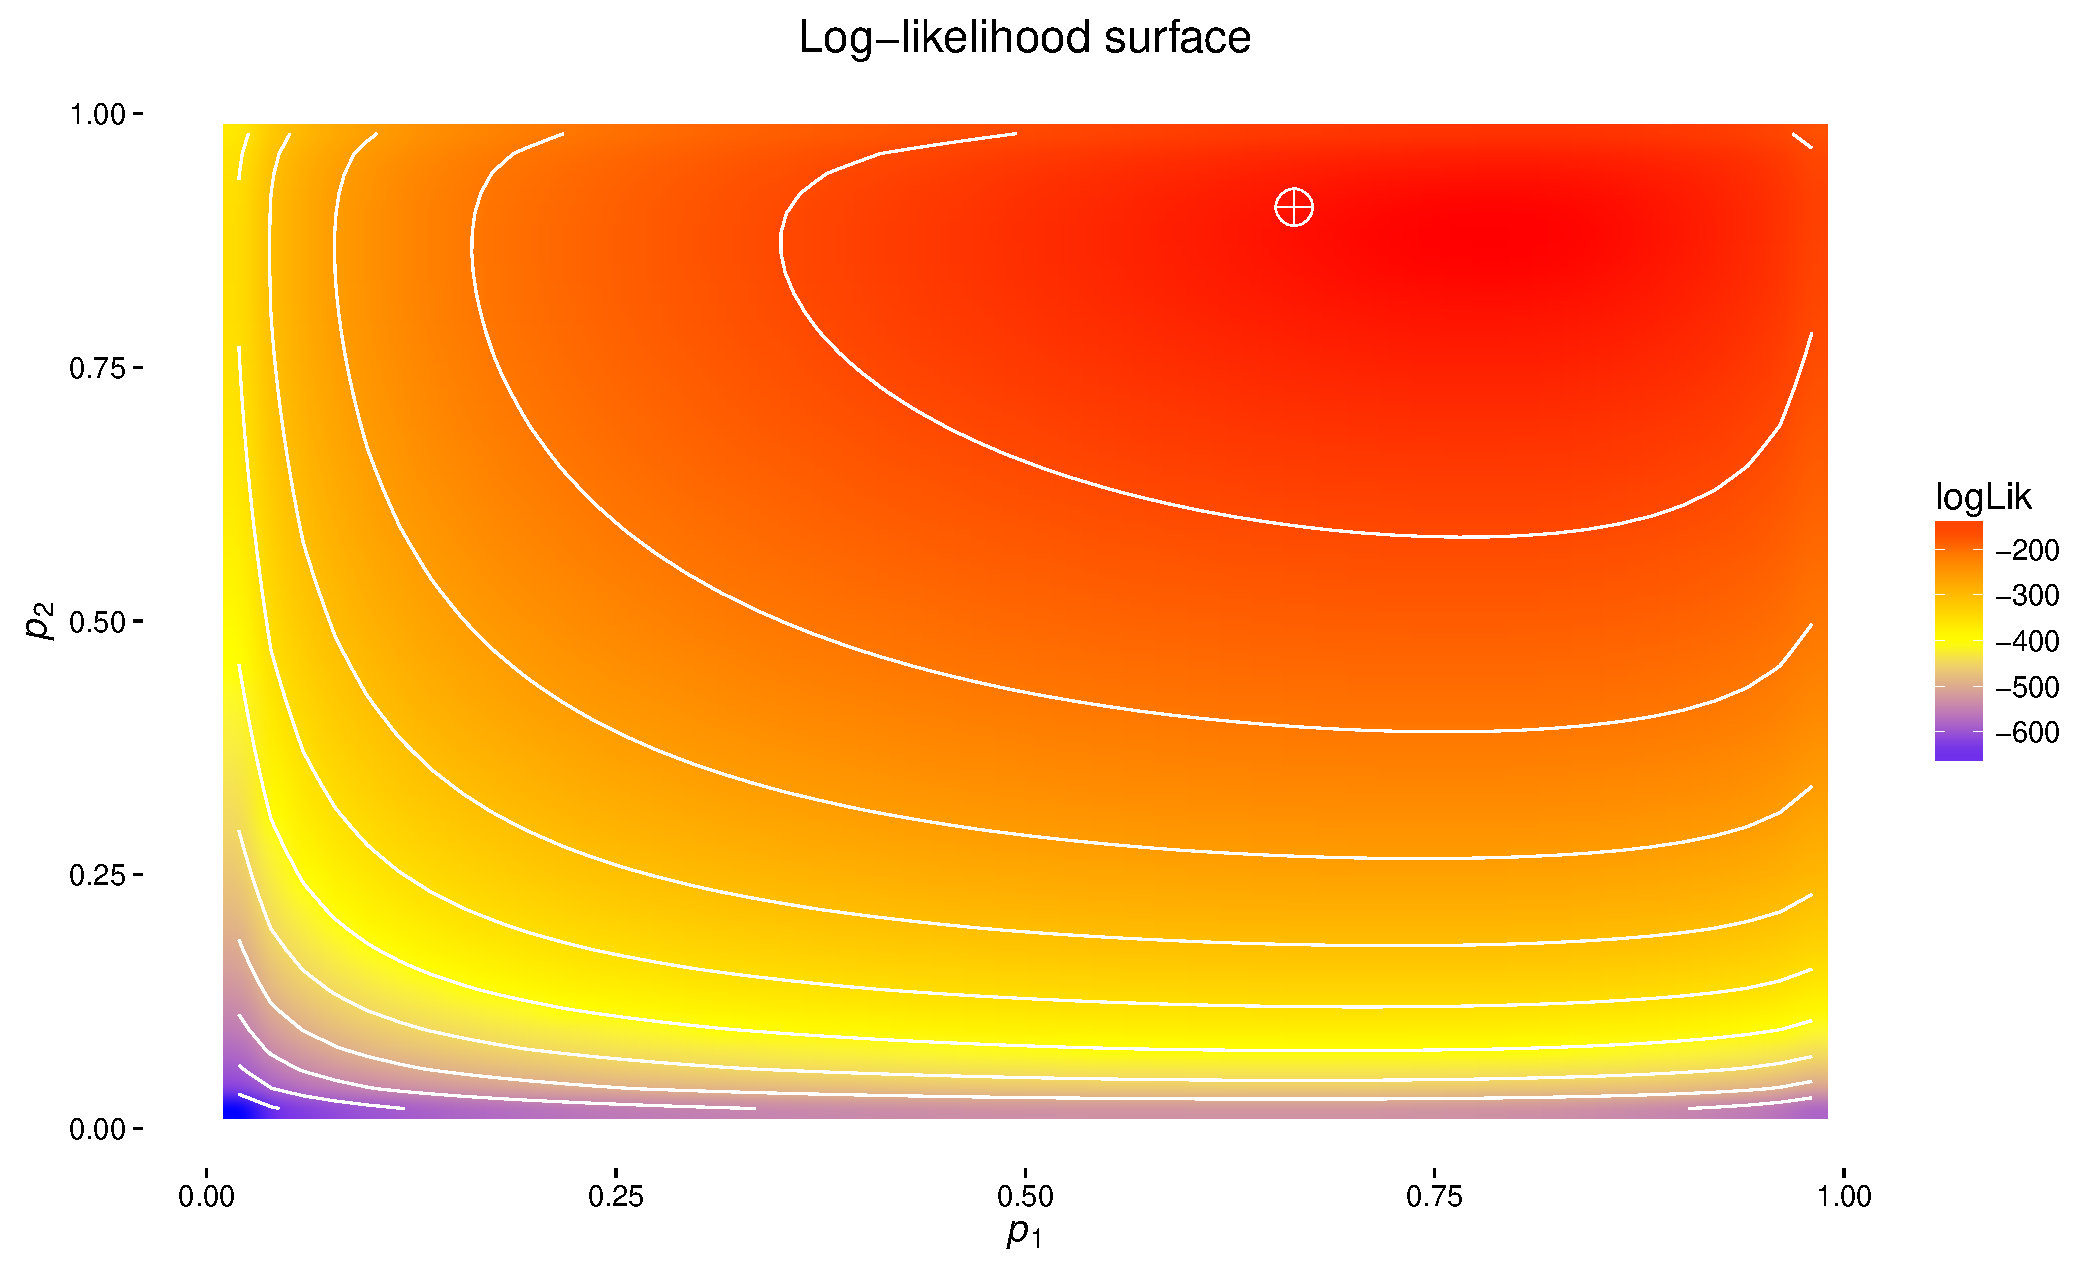
\includegraphics[width=\textwidth]{pdf/freq1-freq2-lik-surf1}}
	\end{center}
\end{frame}
}

{ \setbeamercolor{background canvas}{bg=white!20!black} %\setbeamercolor{math text}{fg=itemcol, bg=itemcol}
\begin{frame}[c,plain]{\setbeamercolor{math text}{fg=itemcol, bg=itemcol}Likelihood surface for $p_1$ and $p_2$: high drift}
	\framesubtitle{$F_{st}=0.5,\, \pi=0.475,\, p_1=0.962,\, p_2=0.343$}
	\begin{center}
		\frame{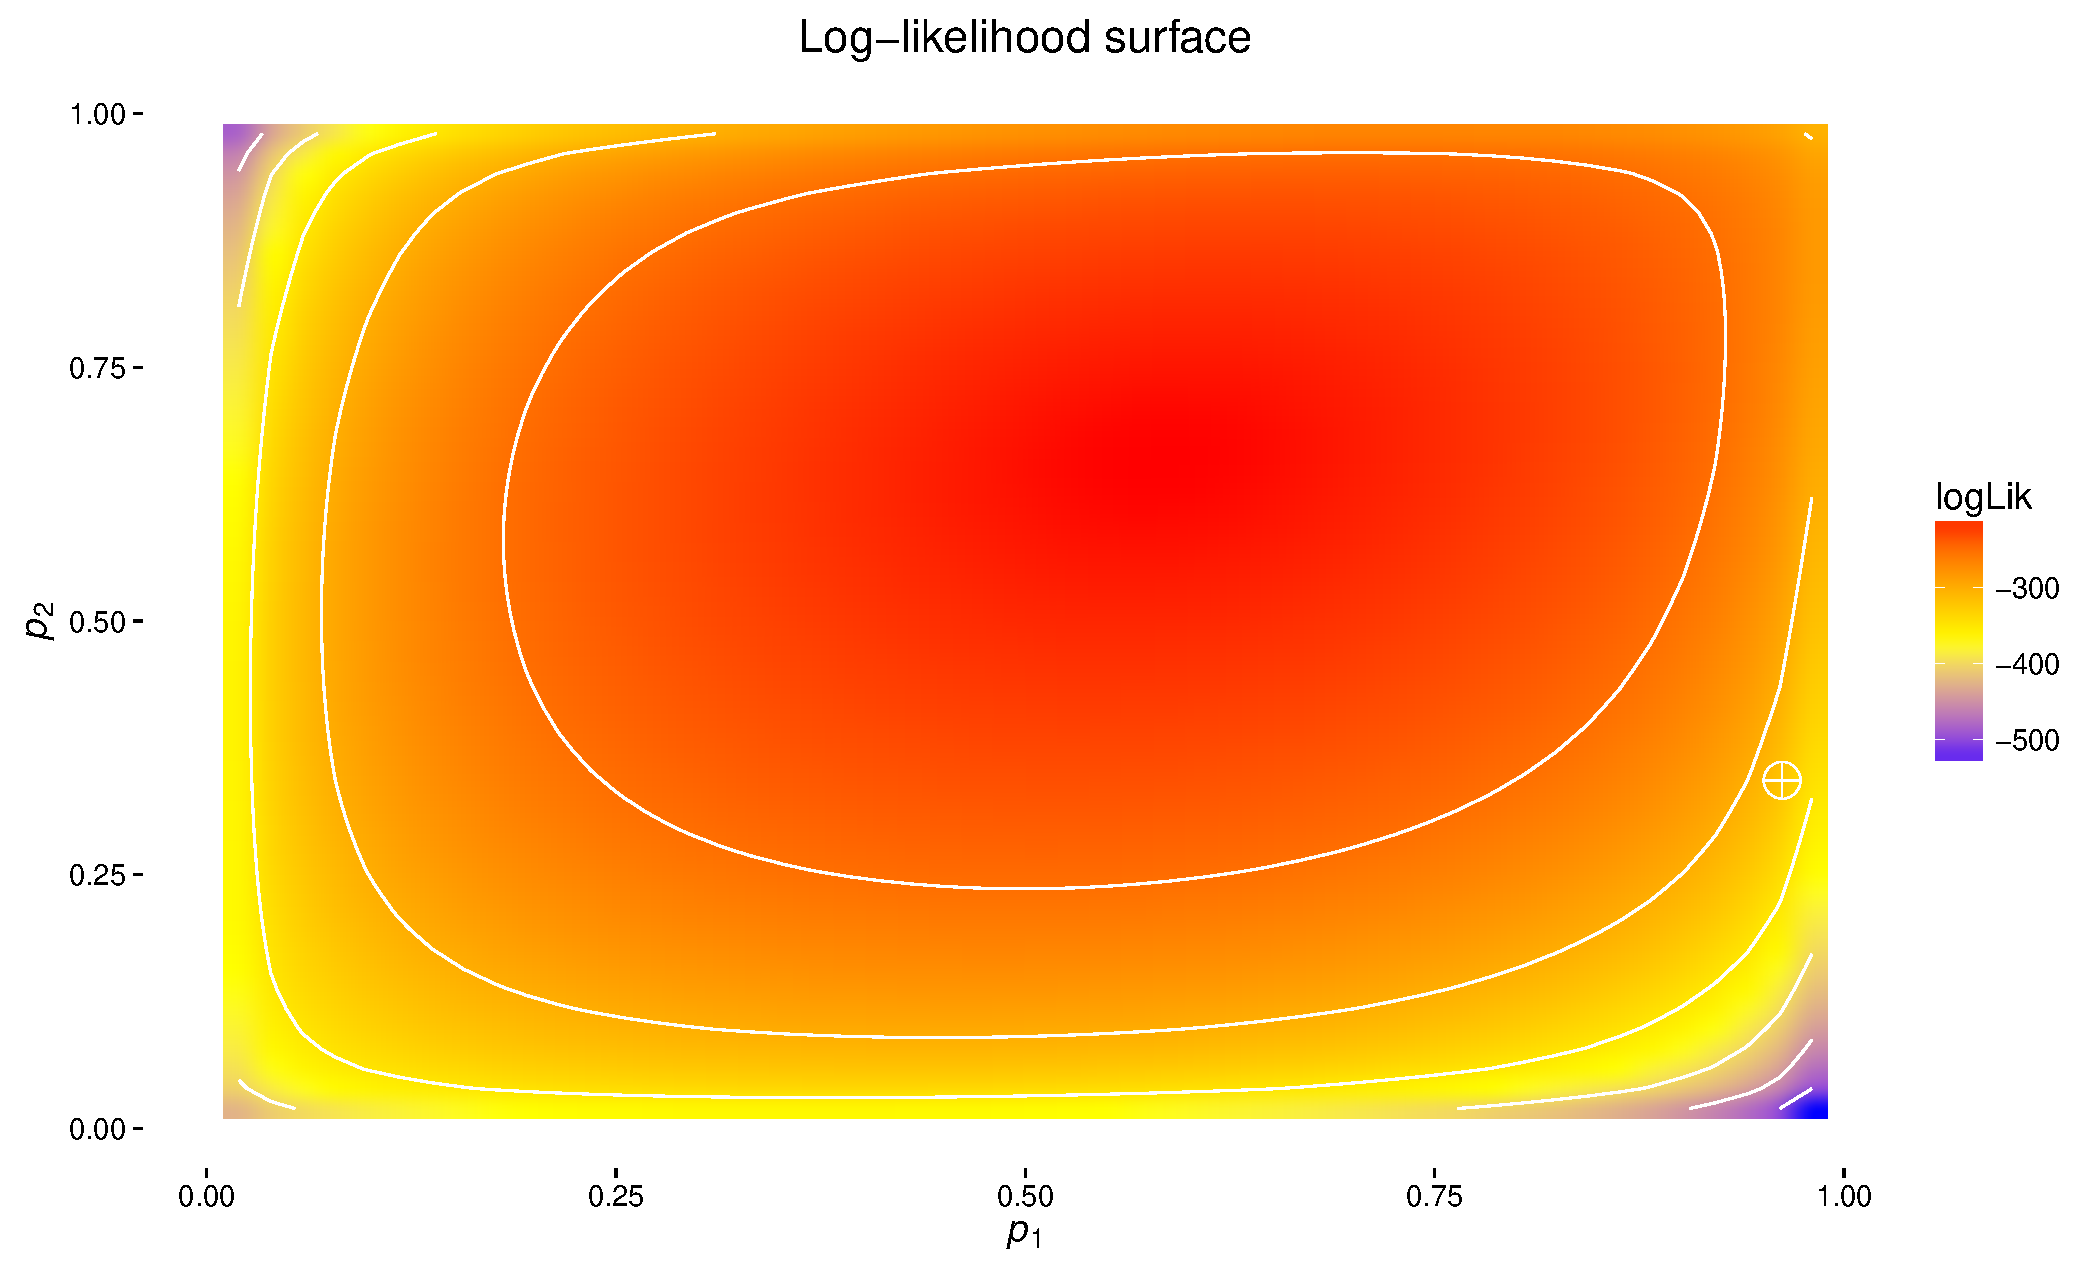
\includegraphics[width=\textwidth]{pdf/freqs1-freqs2-bad-lik-surf1}}
	\end{center}
\end{frame}
}

%{ \setbeamercolor{background canvas}{bg=white!20!black} %\setbeamercolor{math text}{fg=itemcol, bg=itemcol}
%\begin{frame}[c,plain]{\setbeamercolor{math text}{fg=itemcol, bg=itemcol}Likelihood surface for $p_1$ and $p_2$: high drift}
%	\framesubtitle{$F_{st}=0.5,\, \pi=0.922,\, p_1=0.999,\, p_2=0.414$}
%	\begin{center}
%		\frame{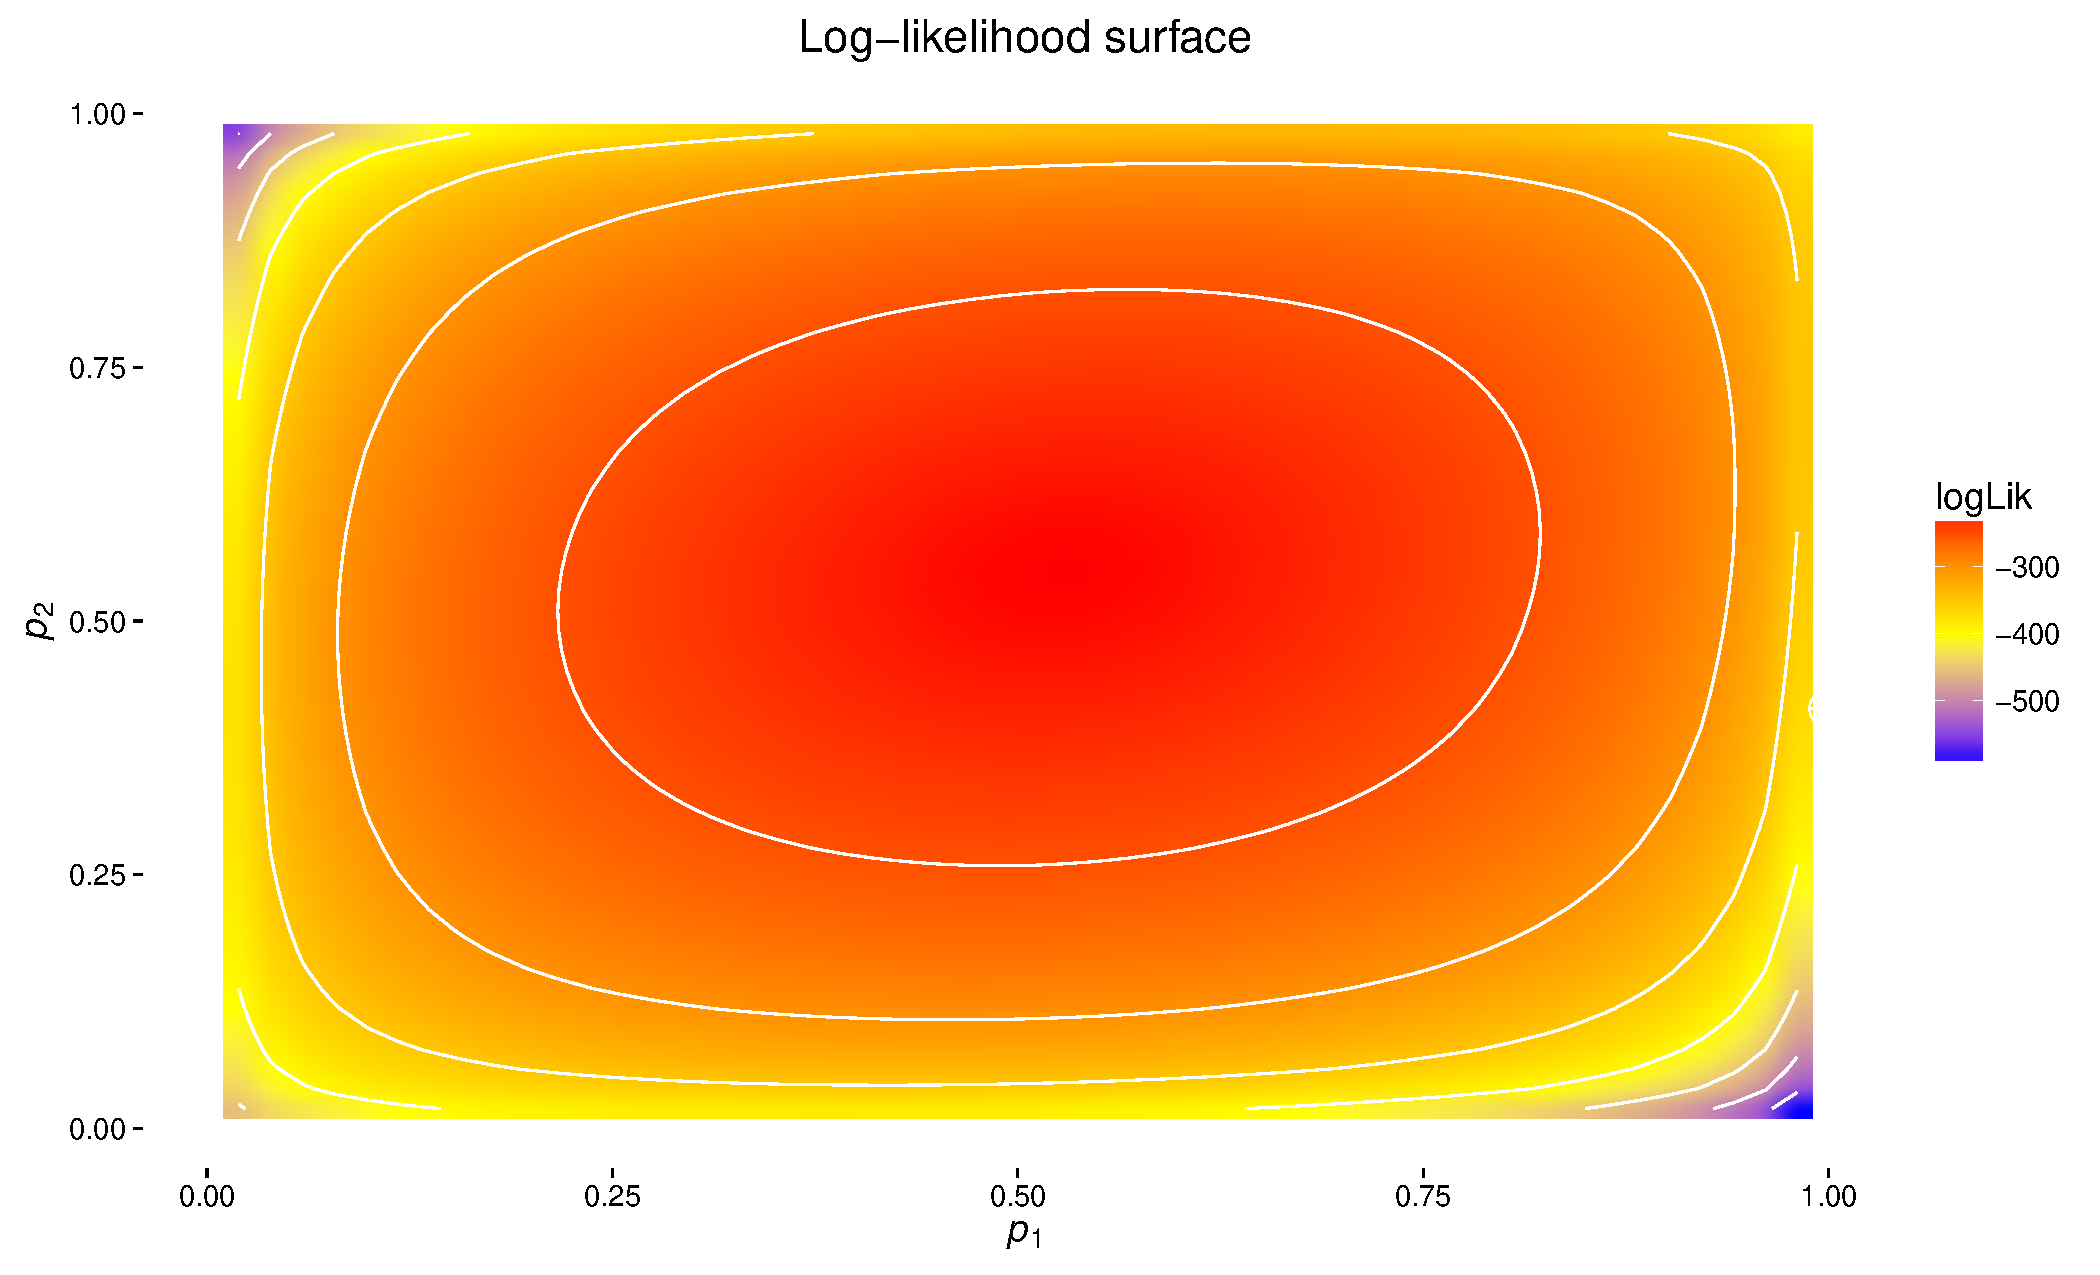
\includegraphics[width=\textwidth]{pdf/freqs1-freqs2-bad-lik-surf3}}
%	\end{center}
%\end{frame}
%}


\begin{frame}[t]{Conclusions and future directions}
	\pause
	\fontsize{10pt}{10}\selectfont
	\begin{enumerate}
		\item{Conclusions:}
		\vspace{0.1in}
		\setlength\itemsep{0.2in}
		\begin{itemize}
			\setlength\itemsep{0.2in}
			\item $F$-models have great potential for helping make inferences in non-model polyploids.
			\item Allopolyploid model works best for closely related subgenomes.
		\end{itemize}
		\pause
		\item{Future directions:}
		\vspace{0.1in}
		\setlength\itemsep{0.2in}
		\begin{itemize}
		\setlength\itemsep{0.2in}
			\item Include parental data in allopolyploid model if available and develop a model selection framework for testing allopolyploid parentage. \pause
			\item Currently developing software to perform inference with these models (plus a few others). Hoping to have a beta version in late summer.
		\end{itemize}
	\end{enumerate}

\end{frame}

\begin{frame}[c]{Code availability}
	\fontsize{10pt}{10}\selectfont
	\begin{itemize}
	\setlength\itemsep{0.3in}

		\item Presentation slides and notes are on fig\textbf{share}.
		
		\item R scripts for the simulations and other code are on GitHub:\\[0.05in]\url{https://github.com/pblischak/evolution2016}.
		
		
	\end{itemize}
	\vspace{0.3in}

	{\Large \alert{Links for everything are in the GitHub repository for this presentation: \textbf{pblischak/evolution2016}.}}
	\vspace{0.2in}

	\hfill {\tiny \#openscience}
\end{frame}

\begin{frame}[t,plain]{Acknowledgments}
  \vspace{0.2in}

  \begin{itemize}
    \setlength\itemsep{0.3in}
    \item John Novembre, Xin He, Matthew Stephens, and their lab members for the opportunity to present at U. of Chicago (and to John Blischak for organizing the visit).
    \item My labmates in the Wolfe and Kubatko labs.
    \item National Science Foundation for funding the larger project that includes the development of the models presented here.
  \end{itemize}

\end{frame}

\begin{frame}[c,plain]{}
	\begin{center}
		{\Huge Thanks!}\\
		\vspace{0.5in}
		{\LARGE Questions?}
	\end{center}
\end{frame}

\end{document}
